\subsubsection*{Analysis}
\begin{tabular}{@{}l l}
\textbf{Scope}:&The AuctionHouse\textsuperscript{TM} automated administration system\\
\textbf{Level}:&User goal\\
\textbf{Primary Actor}:&Secretary\\
\textbf{Stakeholders and Interests}:&\begin{tabular}[t]{@{}l}Secretary: Wants to enter the new customer's parameters easily and quickly.\\Customer: wants to be registered as a regular customer.\end{tabular}\\
\textbf{Preconditions}:&Secretary is identified and authenticated.\\
\textbf{Postconditions}:&\begin{tabular}[t]{@{}l}The customer is registered in the system as a ``regular customer''.\\The customer's address has been added to a mailing list for the auction catalogue.\\If the customer specified a category of interest, their e-mail address has been added to a mailing list for the theme-specific notifications.\end{tabular}\\
\textbf{Special requirements}:&A list of item categories/themes is available in the system\\
\textbf{Frequency of occurence}:& \begin{tabular}[t]{@{}l}READ THE DAMN EMAIL YOU GOT, IDIOT!.\end{tabular}
\end{tabular}\\\\
\textsl{Main Success Scenario}
\begin{enumerate}[noitemsep]
	\item The user starts the `register regular customer' transaction with the system, having all parameters of the item to be added ready.
	\item The system returns a list of item categories
	\begin{itemize}[noitemsep]
		\item The customer's name
		\item The customer's address
		\item The customer's postal code
		\item The customer's city data
		\item Category of interest (optional)
		\item The customers e-mail address (required if the above was provided)
	\end{itemize}
	\item The system registers the new regular customer using the provided parameters and generates a customer ID.
	\item The system add the provided address to the mailing list
	\item If a category of interest was provided, the system adds the the provided e-mail address to the emailing list of that category.
	\item The system returns to the user with a confirmation message containing the generated customer ID, or a failure. 
\end{enumerate}
\textsl{Extensions}
\begin{itemize}[noitemsep]
	\item When a failure is returned, the system state remains unchanged; no customer or parameters were added.
	\item When not all required parameters were provided, the system will first ask the user to provide it until all parameters is provided.
\end{itemize}
\textsl{System Sequence Diagram}
\begin{figure}[H]
	\centering
	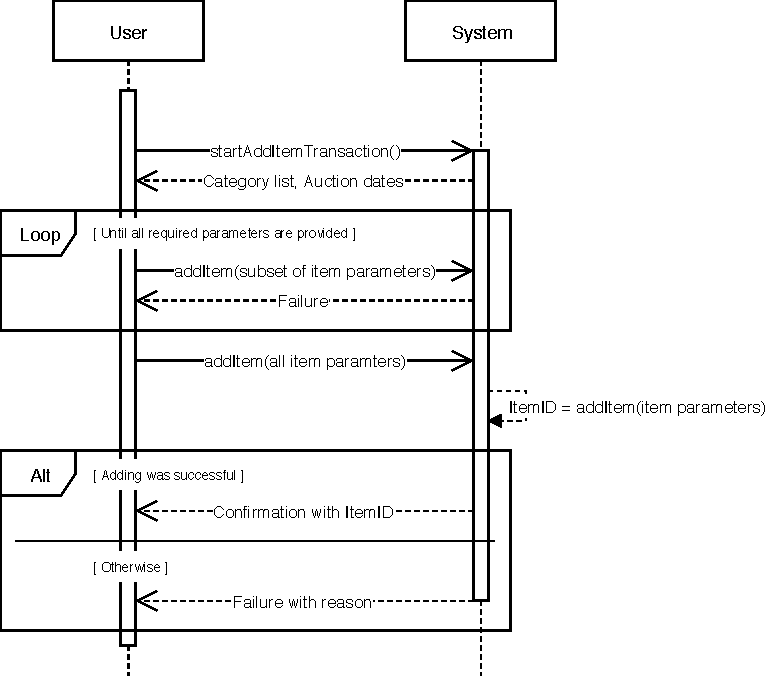
\includegraphics[scale=1]{uml/SD-bb-create.pdf}
	\caption*{Interactions displayed in a System Sequence Diagram defined by the MSS and its extensions in blackbox format}
\end{figure}